\documentclass{beamer}
\usetheme{metropolis}           % Use metropolis theme
\usepackage{arevmath}
\usepackage{varwidth}   
\usepackage{tikz}
\setsansfont[
	  BoldFont={Fira Sans SemiBold},
	    ItalicFont={Fira Sans BookItalic},
		  BoldItalicFont={Fira Sans SemiBold Italic}
		  ]{Fira Sans Book}
\usepackage{xmpmulti}
\usepackage{graphicx}
\def\shrug{\texttt{\raisebox{0.75em}{\char`\_}\char`\\\char`\_\kern-0.5ex(\kern-0.25ex\raisebox{0.25ex}{\rotatebox{45}{\raisebox{-.75ex}"\kern-1.5ex\rotatebox{-90})}}\kern-0.5ex)\kern-0.5ex\char`\_/\raisebox{0.75em}{\char`\_}}}

\DeclareMathOperator{\dist}{dist}
\newcommand{\light}[1]{\textcolor{gray}{#1}}


\title{Efficient Generation of Geographically Accurate Transit Maps}
\date{}
\author{Hannah Bast\,\footnotesize$^1$, \small Patrick Brosi\,\footnotesize$^1$ \small and Sabine Storandt\,\footnotesize$^2$}
\institute{\footnotesize$^1$\,University of Freiburg\\\footnotesize$^2$\,LMU Würzburg\\\\26th ACM SIGSPATIAL - Seattle, Washington, USA}
\begin{document}
\maketitle
\begin{frame}{Motivation}
	\begin{tikzpicture}[overlay]
		\node at (1.5, 3.2) {Official CTA map};
	    \node at (1.5, 0) {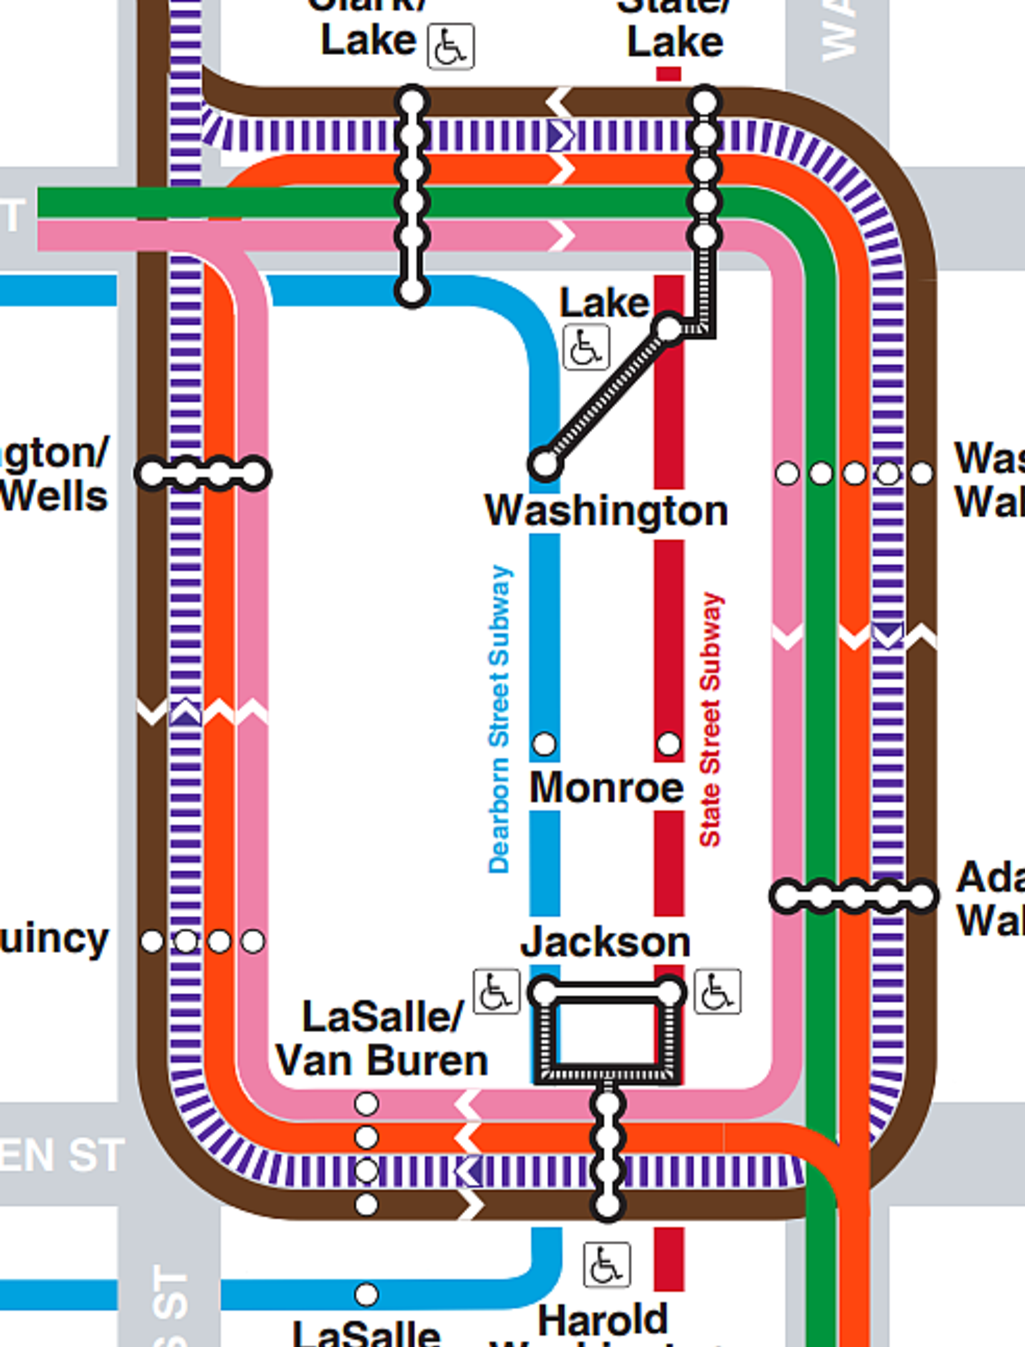
\includegraphics[width=0.3\paperwidth]{figures/chicago_loop.pdf}};
	    \pause
	    \node at (5.5, 3.2) {HERE};
	    \node at (5.5, 0) {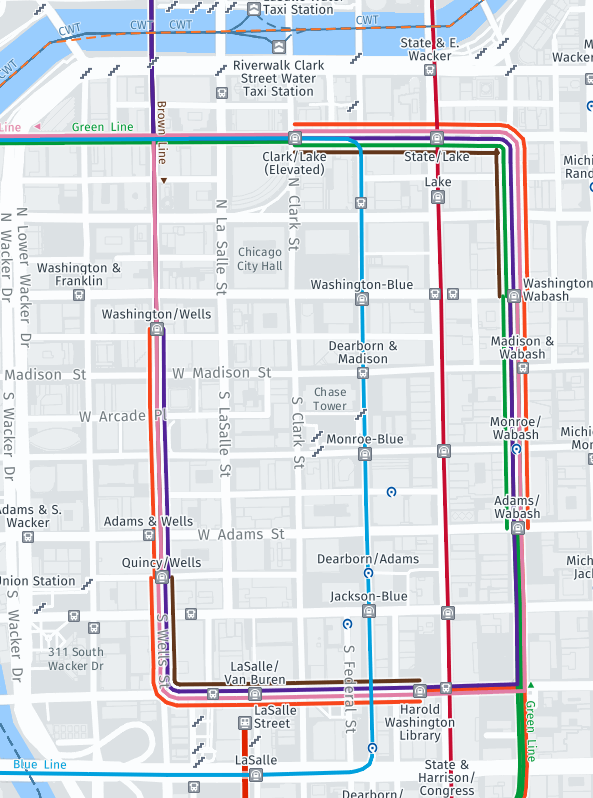
\includegraphics[width=0.3\paperwidth]{figures/chicago_here.png}};
	    \pause
	    \node at (9.5, 3.2) {Google};
	    \node at (9.5, 0) {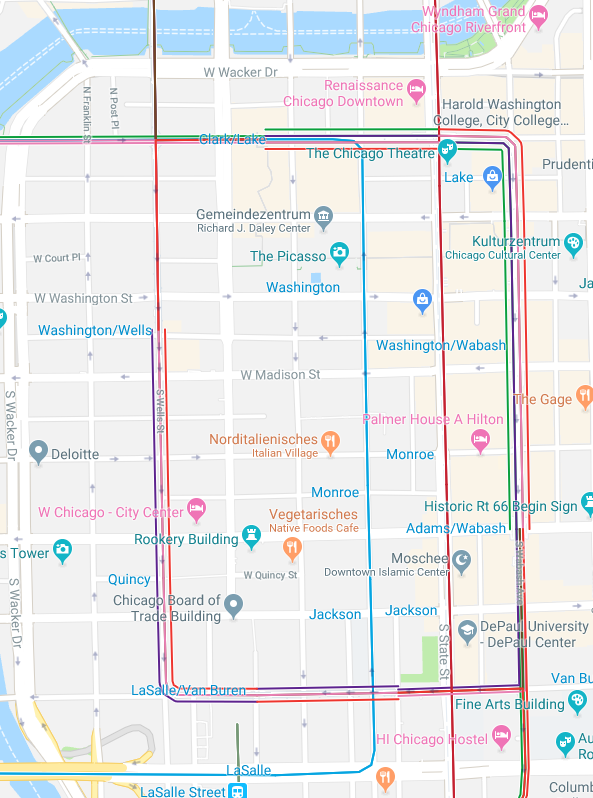
\includegraphics[width=0.3\paperwidth]{figures/chicago_google.png}};
	\end{tikzpicture}
\end{frame}

\begin{frame}{Challenges}
	\begin{tikzpicture}[xshift=.2cm, yshift=.4cm, overlay]
		\begin{scope}[yshift=1.5cm]
			\node at (0.3, 1.7) {\small Official};
			\node at (2.6, 1.7) {\small HERE};
			\node at (4.9, 1.7) {\small Google};

			\node[circle, draw=black!60!green, line width=1pt,inner sep=0.7cm, path picture={\node at (path picture bounding box.center) at (-2.09, 1.5) {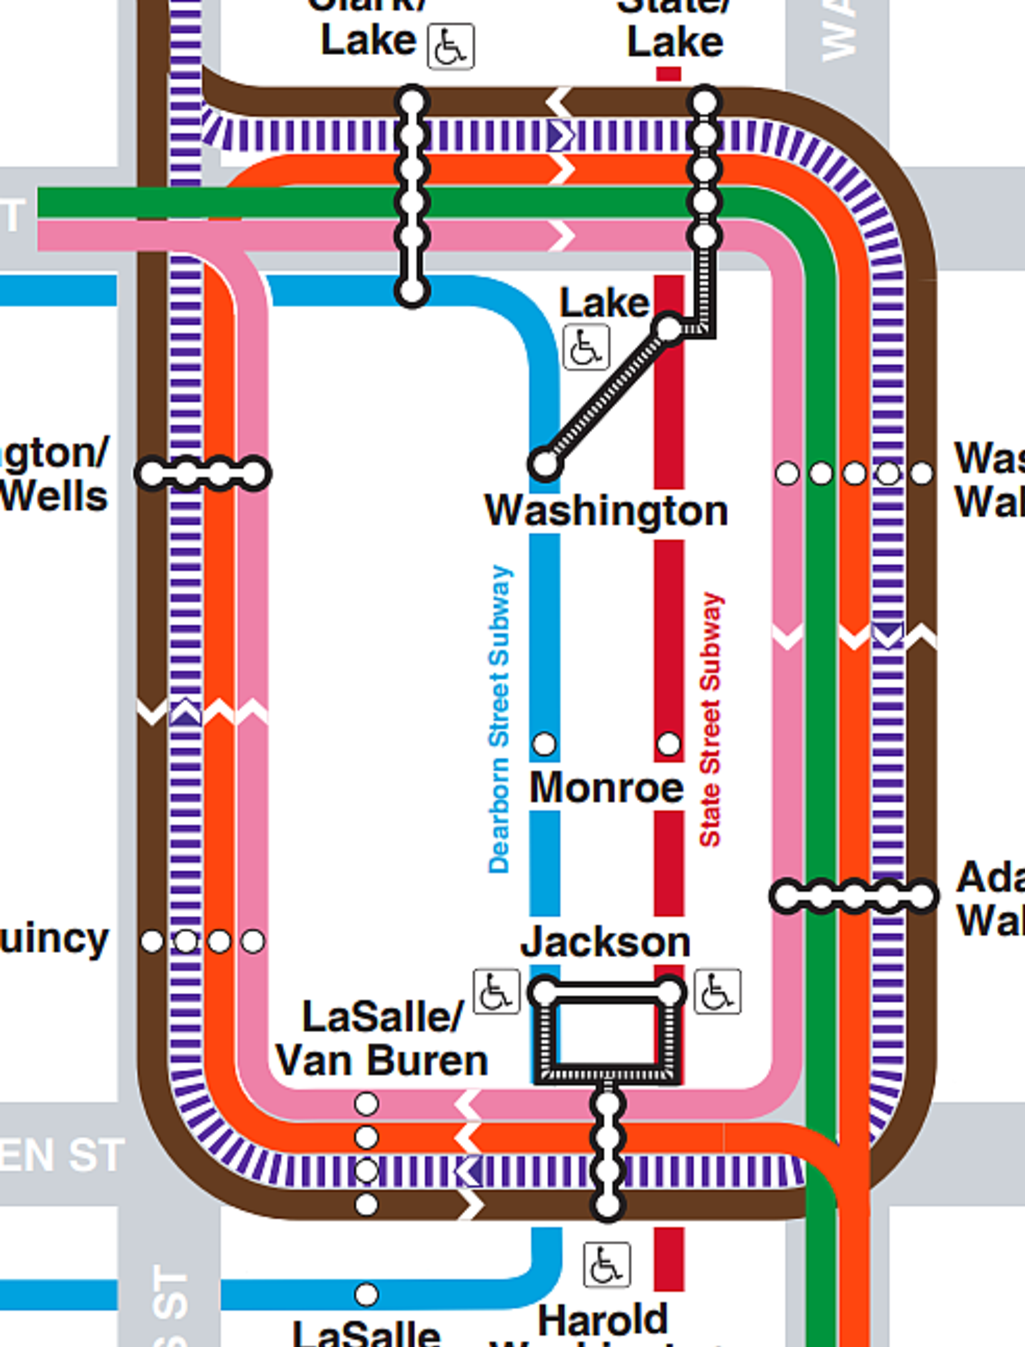
\includegraphics[width=6.5cm]{figures/chicago_loop.pdf}};}] at (0.3, 0) {};
			\node[circle, draw=black!40!red, line width=1pt, inner sep=0.7cm, path picture={\node at (path picture bounding box.center) at (-4.45, 3) {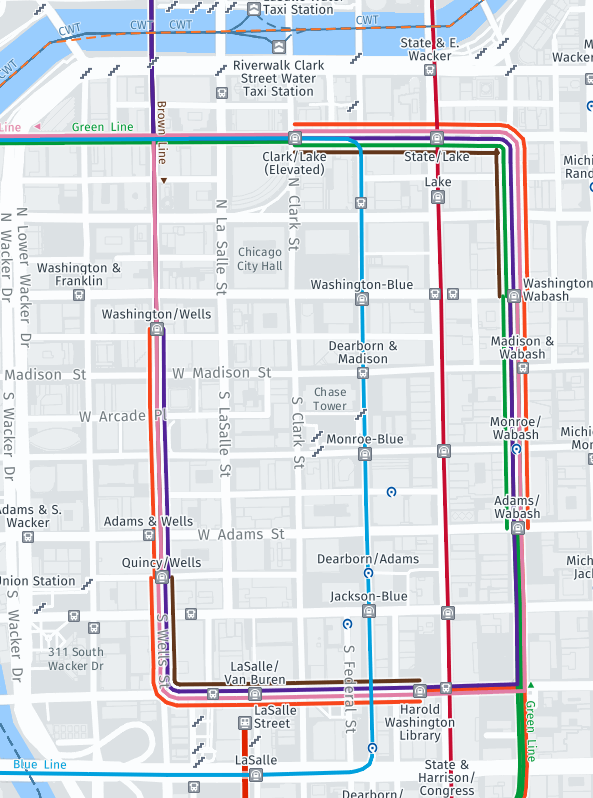
\includegraphics[width=12cm]{figures/chicago_here.png}};}] at (2.6, 0) {};
			\node[circle, draw=black!40!red, line width=1pt, inner sep=0.7cm, path picture={\node at (path picture bounding box.center) at (-4.45, 3) {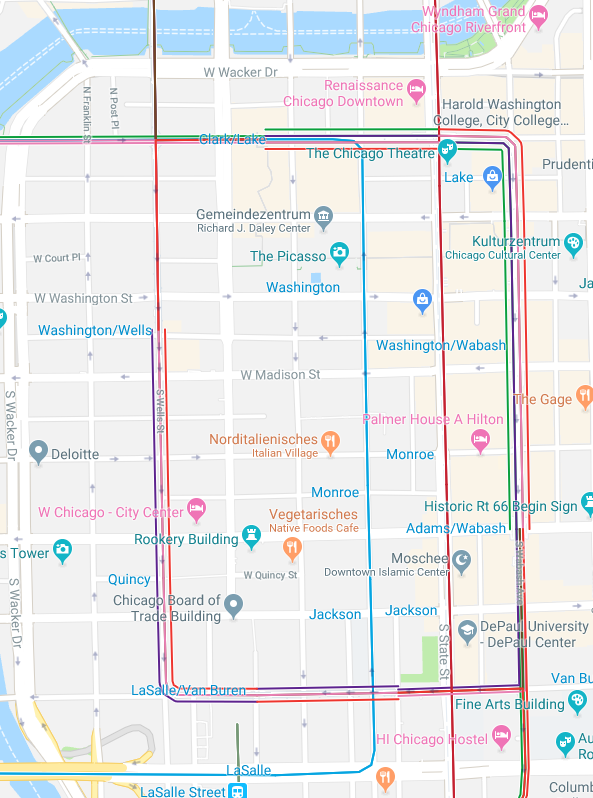
\includegraphics[width=12cm]{figures/chicago_google.png}};}] at (4.9, 0) {};

			\node at (11.3, 0) {
			\vbox{\begin{varwidth}{0.5\textwidth}
				\begin{itemize}
					\item Avoid overlapping lines
				\end{itemize}
			\end{varwidth}}};
		\end{scope}

		\pause

		\begin{scope}[yshift=-1.0cm]
			\node[circle, draw, inner sep=0.7cm, path picture={\node at (path picture bounding box.center) at (-1.387, -3.25) {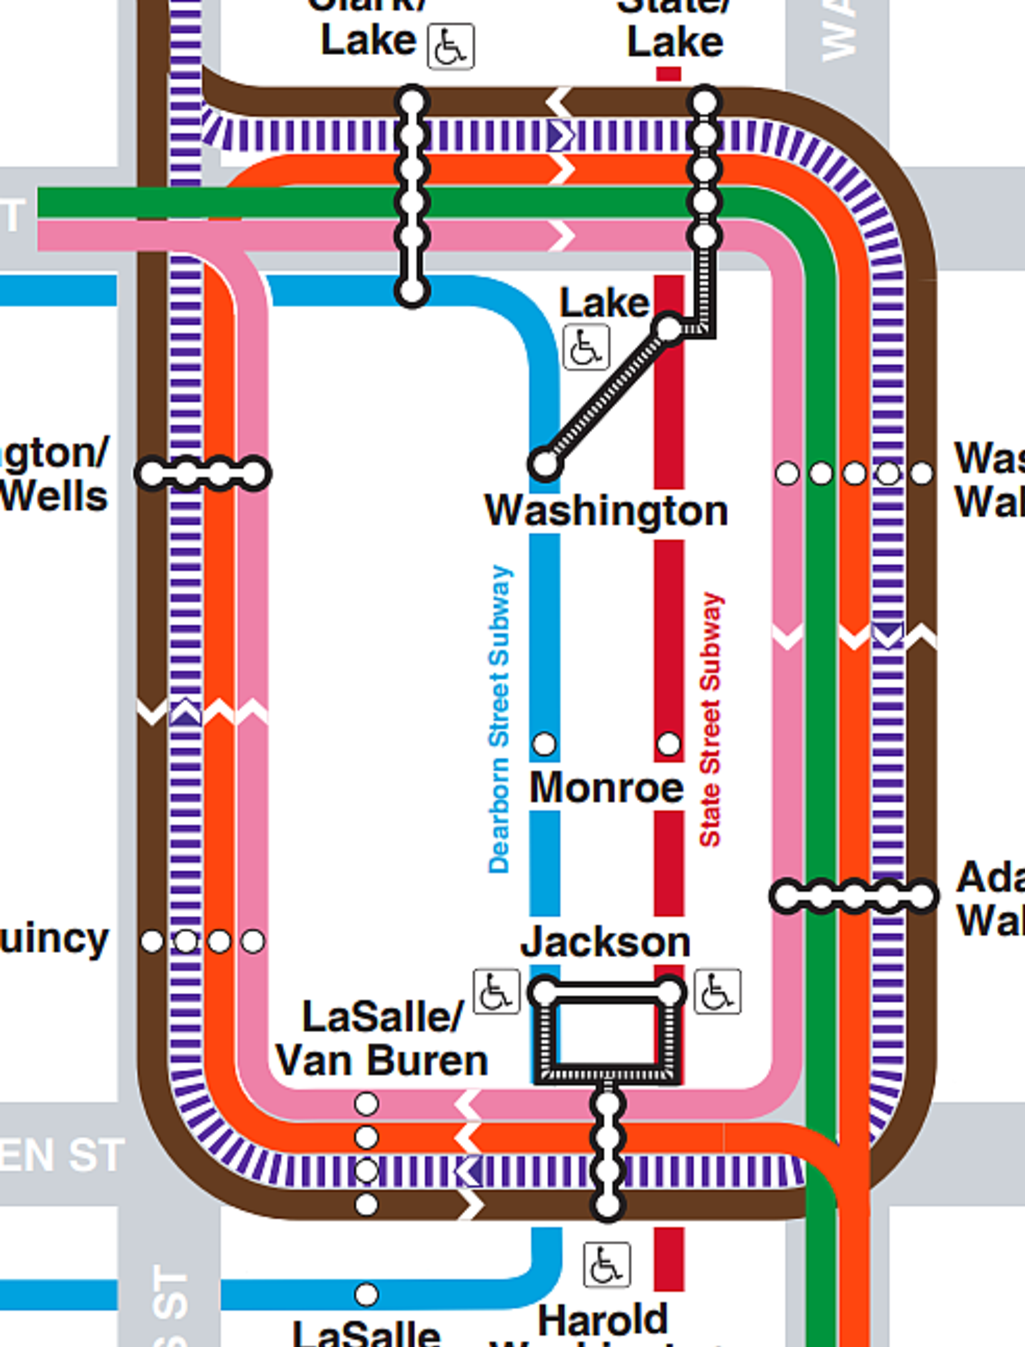
\includegraphics[width=6.75cm]{figures/chicago_loop.pdf}};}] at (0.3, 0) {};
			\node[circle, draw, inner sep=0.7cm, path picture={\node at (path picture bounding box.center) at (-3.75, 8.9) {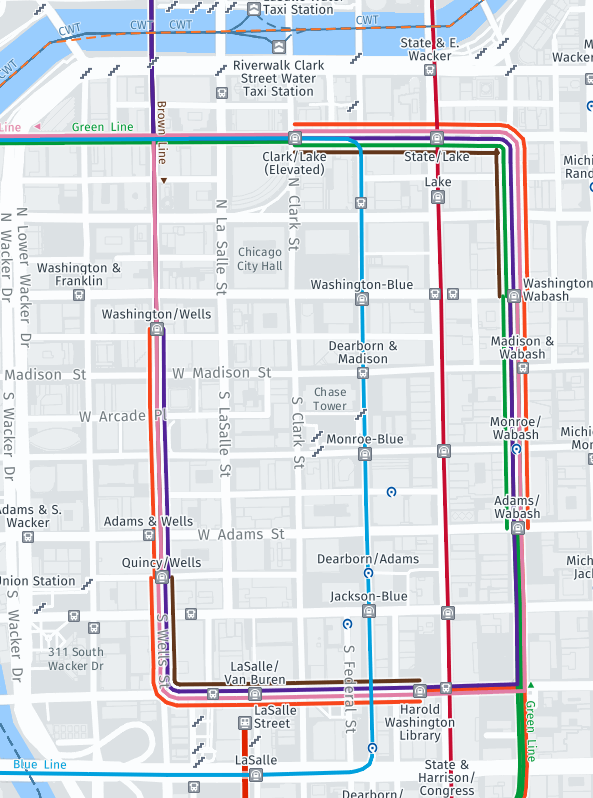
\includegraphics[width=18cm]{figures/chicago_here.png}};}] at (2.6, 0) {};
			\node[circle, draw, inner sep=0.7cm, path picture={\node at (path picture bounding box.center) at (-4.25, -7.9) {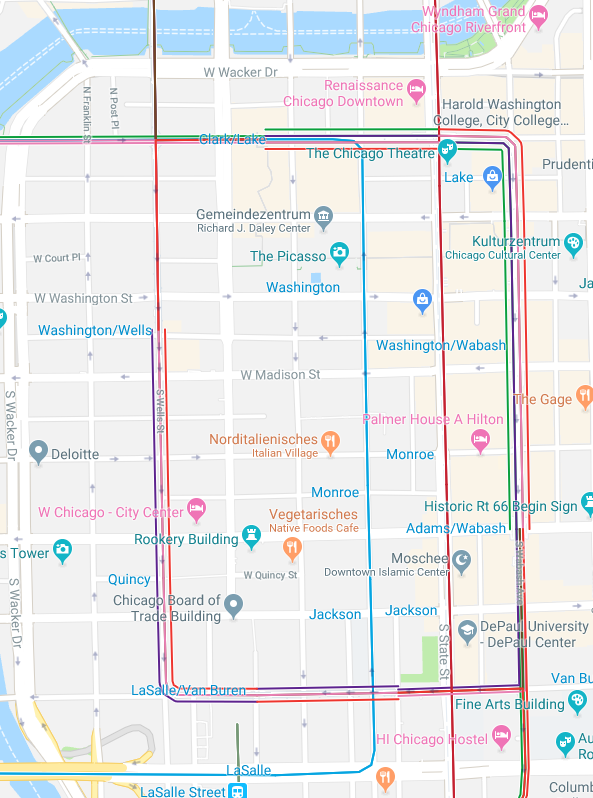
\includegraphics[width=18cm]{figures/chicago_google.png}};}] at (4.9, 0) {};
			\node at (11.3, 0) {
			\vbox{
				\begin{itemize}
					\item Match line orderings
				\end{itemize}
			}};
		\end{scope}

		\pause

		\begin{scope}[yshift=-3.5cm]
			\node[circle, draw, inner sep=0.7cm, path picture={\node at (path picture bounding box.center) at (-2.03, 2.9) {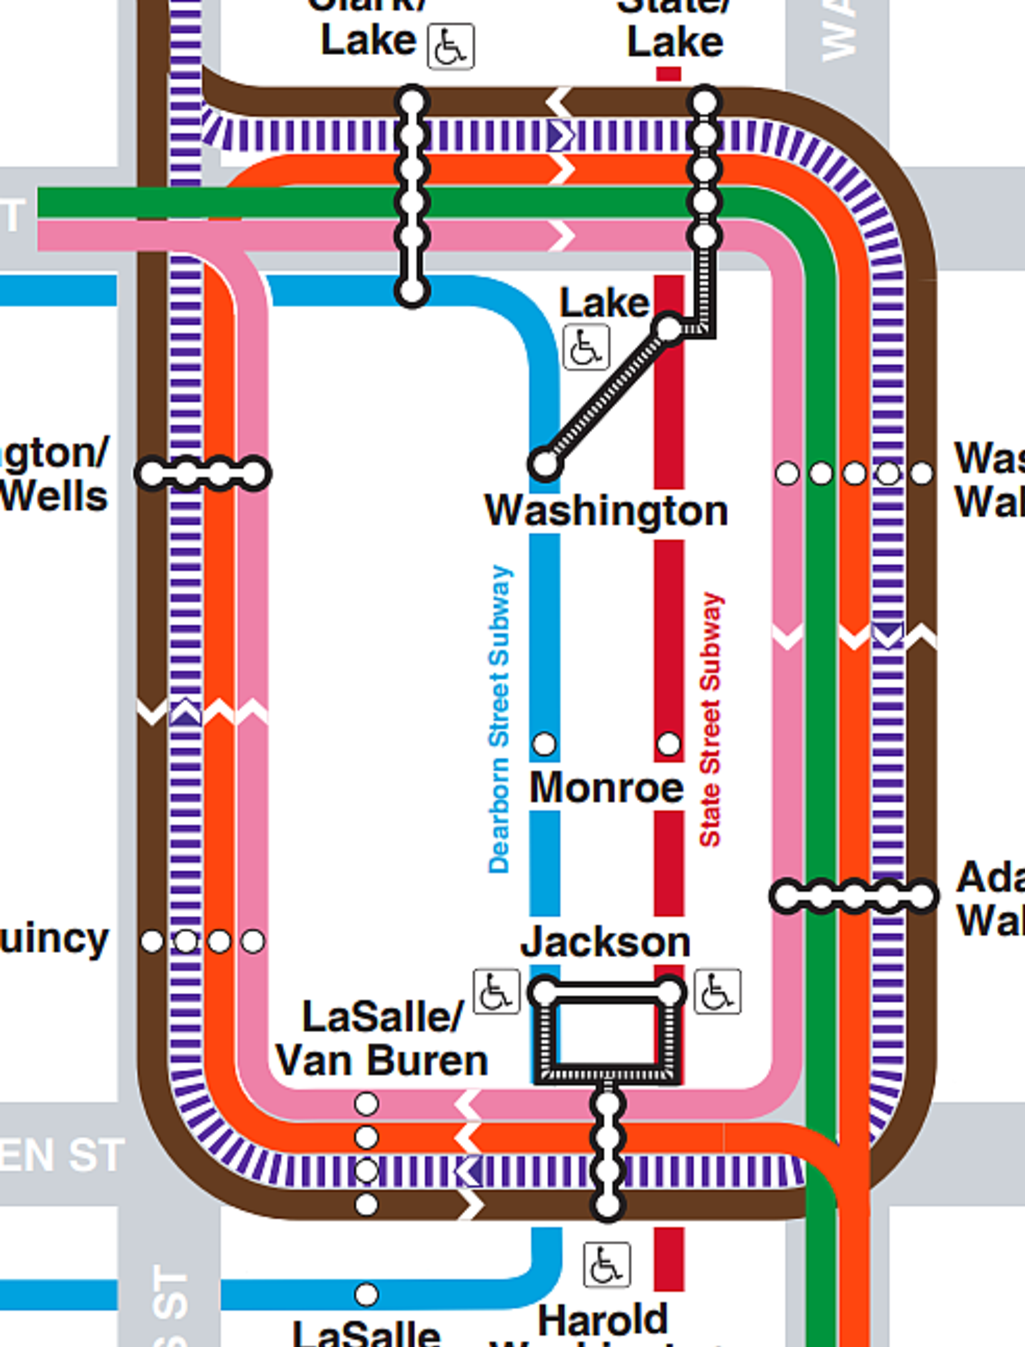
\includegraphics[width=6.5cm]{figures/chicago_loop.pdf}};}] at (0.3, 0) {};
			\node[circle, draw, inner sep=0.7cm, path picture={\node at (path picture bounding box.center) at (-6.75, 8.9) {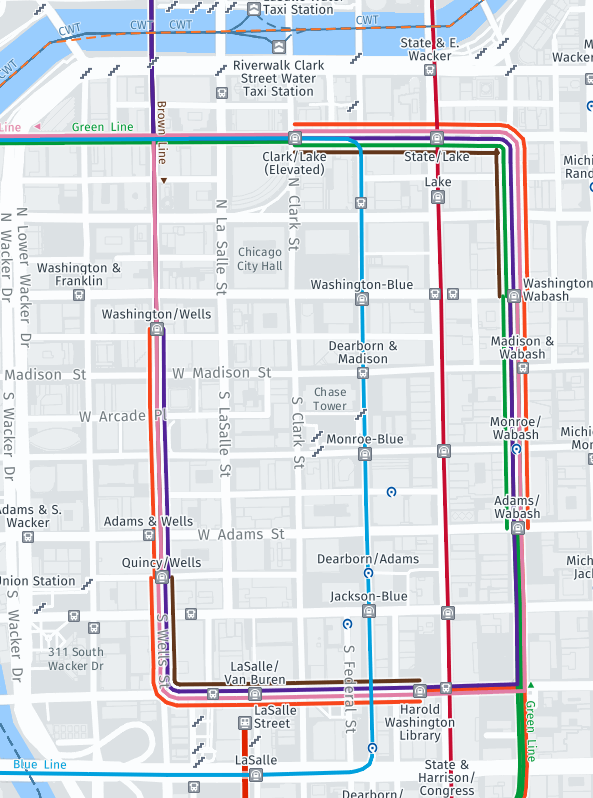
\includegraphics[width=18cm]{figures/chicago_here.png}};}] at (2.6, 0) {};
			\node[circle, draw, inner sep=0.7cm, path picture={\node at (path picture bounding box.center) at (-6.75, 8.9) {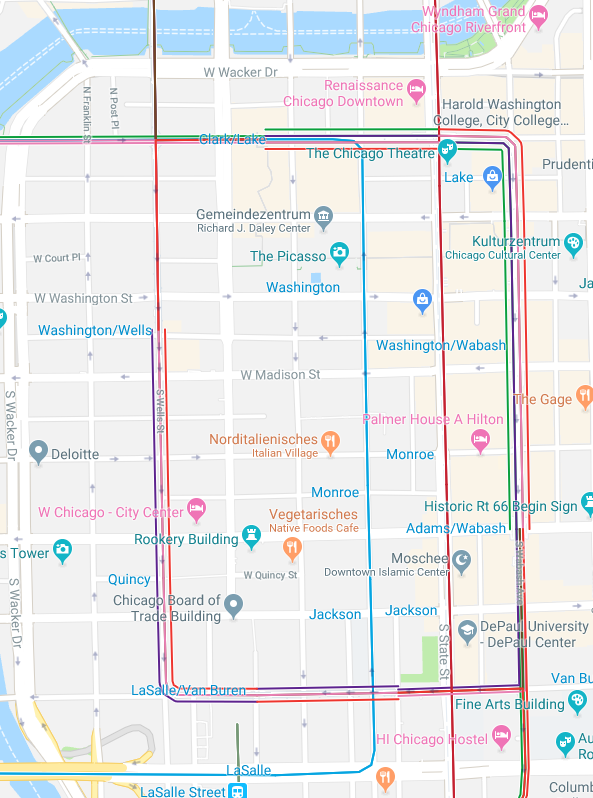
\includegraphics[width=18cm]{figures/chicago_google.png}};}] at (4.9, 0) {};
			\node at (11.3, 0) {
			\vbox{\begin{varwidth}{0.5\textwidth}
				\begin{itemize}
					\item Clearly indicate line continuations
				\end{itemize}
			\end{varwidth}}};
		\end{scope}

	\end{tikzpicture}
\end{frame}




\end{document}
